\section[General]{General
\footnote{
  $CVS~revision~ $Id: a-intro.tex,v 1.2 2003/11/18 19:52:19 lerose Exp $ $ 
}
\footnote{Authors: J.LeRose \url{mailto:lerose@jlab.org}}
} 

 This document contains the following information concerning the Hall
 A ``base equipment'':
 \begin{list}{--}{\setlength{\itemsep}{0.cm}}
    \item safety assessment 
    \infolevone{\item technical overview} 
    \infolevtwo{\item operating procedures} 
    \infolevthree{\item performance information}
 \end{list}

\infolevtwo{
  The operating procedures are intended to
  provide shift personnel with the information they need to
  understand, at least at a rudimentary level, the function of the
  various subsystems in the end-station. It should also aid in
  determining if the equipment is performing properly and provide
  instructions for what to do in the case of malfunctions. This
  document is not intended to be a comprehensive reference but is
  rather a guide for the use of on shift personnel. When appropriate,
  other references are indicated for the user who requires more
  information.  
}

  It is assumed that the reader of this document has
  been through all the required Jefferson Lab safety training. Hence,
  the material covered in those courses is for the most part not
  repeated here. End-station specific safety items are covered in
  ``The Experiment Safety Assessment Document for the Hall A Base
  Equipment'' which is required reading for all shift personnel.  This
  document also contains some safety information when deemed
  appropriate.
	
%\infolevthree{  
%  A CAD-drawn view of Hall A and its basic equipment is shown
%  on Fig.\ref{fig:cad_halla_1}.
%\begin{figure}[tbh]
%\begin{center}
%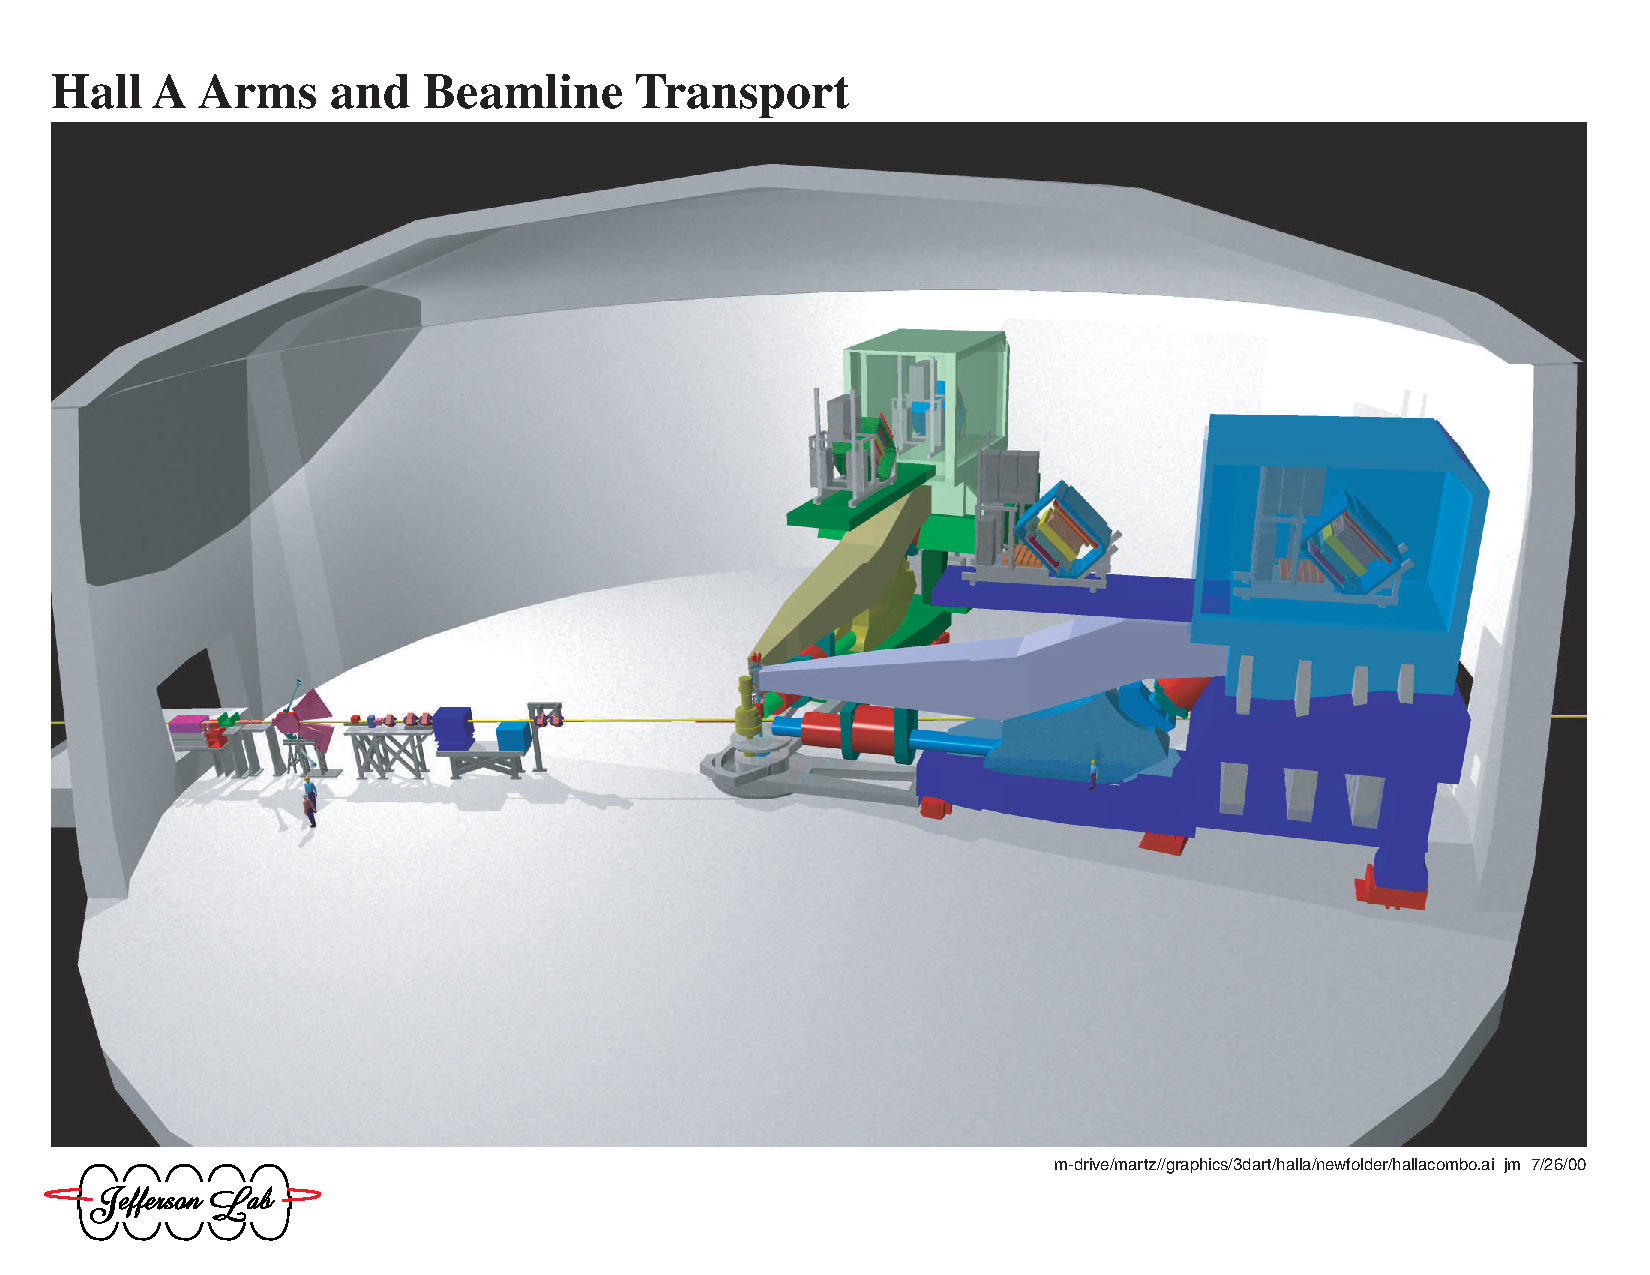
\includegraphics[angle=0,width=\textwidth]{hallacombo}
%\caption[Hall A CAD-drawn picture]
%   {Hall A CAD-drawn picture.}
%\label{fig:cad_halla_1}
%\end{center}
%\end{figure}
%}

\begin{safetyen}{10}{15}
\section{The Personnel Safety System} 
\end{safetyen}

 Users and staff working on the accelerator site are protected from
 the dangers associated with the prompt ionizing radiation that the
 accelerator beam produces by the Personnel Safety System or PSS.  The
 PSS keeps ionizing radiation out of areas where people are working,
 and keeps people out of areas where ionizing radiation is present.

 There are a total of five states for the Hall~A Personnel Safety
 System: Restricted Access, Sweep, Controlled Access, RF Power Permit,
 and Beam Permit.

\begin{safetyen}{10}{10}
\subsection{Restricted Access}
\end{safetyen}
 
 Restricted Access is the PSS system state when delivery of beam
 and/or RF power is not permitted, and entry to and exit from the hall
 is not controlled by the Personnel Safety System.  This is the normal
 state of the hall when the accelerator is off and no experiments are
 running.  Access is ``restricted'' only in the sense that the hall is
 not open to the general public.

\begin{safetyen}{10}{10}
\subsection{Sweep}
\end{safetyen}

Sweep is the state of the PSS when delivery of beam and/or RF power is
not permitted and access is limited to the Jefferson Lab personnel
conducting the sweep operation.  The hall's entrance gates are closed
from the inside to ensure that no one can enter behind the person
conducting the sweep. During the sweep, an Assigned Radiation Monitor
or ARM systematically searches the hall to verify the absence of
people and to arm the run/safe boxes. The ARM posts a guard at the
entrance to the hall as another method of ensuring that no one enters
after him.
 
When the Assigned Radiation Monitor is ready to perform a sweep, the
Machine Control Center or MCC must first place the hall in the Sweep
state. The Personnel Safety System will read ``Sweep In Progress."
Once the hall is placed in the sweep state, the sweep monitors enter
the first gate to the hall, making sure it locks behind them. The ARM
then notifies the MCC that he is ready to begin the sweep. The MCC
communicates with the sweep monitors via intercom and video
camera. Using the video camera, the MCC makes sure both sweep monitors
are wearing the proper dosimetry. At this point the ARM also indicates
that he is in possession of the key needed to arm the Run/Safe boxes
placed throughout the hall.  Having confirmed that the dosimetry is
adequate, the MCC will unlock the second entrance gate allowing the
sweep monitors to enter the hall. Once the sweep monitors pass through
the second gate, they close the gate and ensure it is locked. The
sweep monitors then proceed to the hall entrance where one sweep
monitor is left to guard the entrance and the other begins the sweep.
During the actual sweep, the ARM walks through every area and secluded
workspace in the hall to ensure that no one could be left inside when
the Personnel Safety System moves from the sweep state to controlled
access, power permit, and finally beam permit state. Once he checks an
area, he arms the run/safe box in that area.  After all areas of the
hall have been checked and the run/safe boxes armed, the sweep
monitors will return to the entrance where the sweep began. Before
arming the last run/safe box, the ARM will contact the MCC. Upon
contact, the MCC will check to see if the sweep has ``dropped"; if all
is well he will notify the ARM that it is okay to arm the box. Once
the box is armed, the sweep monitors have 30 seconds to exit both
gates or the sweep will drop, and the entire sweep process will have
to be repeated. After exiting, the ARM must contact the MCC to let
them know the Hall~can now be moved to the controlled access state.
 
\begin{safetyen}{10}{10}
\subsection{Controlled Access}
\end{safetyen}

 Controlled Access is the state of the PSS when delivery of beam
and/or RF power is not permitted but the hall is considered a
controlled area.  In this state, people are ``counted'' both entering
and leaving the hall to ensure that no one is left inside when the
Personnel Safety System advances to the RF Permit or Beam Permit
states.  Hall entry during the controlled access state is permitted
only to people authorized or qualified by Jefferson Lab .  Entry to
and exit from the hall is controlled from the MCC.  The Hall~cannot be
placed in the ``controlled access'' state without having first been
swept.

\begin{safetyen}{10}{10}
\subsection{RF Power Permit} 
\end{safetyen}

When the PSS is in RF Power Permit the hall is considered an
``exclusion area''.  Delivery of RF power is permitted, but beam
delivery is not.  Reaching this state requires that the hall has
passed through the controlled access state and that no one is left
inside the hall. This is usually a temporary state bridging the
transition from the Controlled Access to the Beam Permit state. Once
the Personnel Safety System reads ``Power Permit'', a steady klaxon
sounds in the hall. If you are in the hall when this klaxon sounds,
press the emergency safe button on the nearest run/safe box and
immediately exit the hall. The hall entrance gates are locked at this
time, but there is an emergency exit button at each gate which will
allow you to exit. A four-minute delay is built in between the
transition from RF Power Permit to Beam Permit.
 
\begin{safetyen}{10}{10}
\subsection{Beam Permit}
\end{safetyen}

 When delivery of beam and RF power is permitted to the exclusion area
the PSS state is Beam Permit.  Reaching this state requires having
passed through the RF Power Permit state.

\begin{safetyen}{10}{10}
\subsection{ Run Safe Boxes}
\end{safetyen}

The Personnel Safety System includes Run/Safe boxes which are located
throughout Hall A, and approximately every 100 feet in the linac. A
run/safe box has three positions: Safe, Operational, and Unsafe. When
the hall is in Restricted Access, the run/safe box will be in the Safe
position. While in this position, the PSS prevents delivery of beam to
the hall. Before beam can be delivered, the hall must be swept to
ensure that no one is left inside. During the Sweep, each run/safe box
is moved to the Operational position in preparation for Beam
Permit. After the sweep has been completed and the hall is placed in
the RF Power Permit state, the run/safe box will show Unsafe. Each box
has an emergency stop button. If you see the box in the Unsafe
position, you are in danger of receiving high levels of ionizing
radiation. Immediately press the emergency stop button, exit the hall,
and call the Machine Control Center Crew Chief at extension 7050.

\begin{safetyen}{10}{10}
\section{Hall~A Access} 
\end{safetyen}

Access to Hall~A is governed by the ``Jefferson Lab Beam Containment
Policy and Implementation'' document. This document can be found in
the Jefferson Lab ES\&H Manual (Section 6310, Appendix T2). Work in
designated radiation areas will be governed by the Jefferson Lab
RadCon Manual.  Access procedures during Research Operations depend on
the number of individuals who will be entering the hall and the length
of time they are expected to be there.  A controlled access is used
when a few individuals require entry for a short period of time. If
the hall must be open for an extended period and many people will
enter, then you should use the restricted access procedure instead of
the controlled access procedure.  Normally, when requesting a
controlled access, the hall will be in either the Beam Permit or RF
Permit State - for example, if the beam has been on or it could be
shortly.  If the hall is not already in the Controlled Access state
when you wish to access it, you must request a change to that state
from the Machine Control Center at extension 7050 and indicate that
you intend to make a Controlled Access. The MCC will then send an
Assigned Radiation Monitor to survey the hall. Before anyone enters
the hall, the ARM will carry out a radiation survey and post radiation
areas. Subsequent entry by individuals during the same Controlled
Access period does not require an ARM survey.

\begin{safetyen}{10}{10}
\subsection{Controlled Access Procedure} 
\end{safetyen}

To make a controlled access when the hall is in the controlled access
state, first contact the MCC. The MCC will unlock the first gate at
the entrance to the hall. Once inside, the MCC will release the master
key. Remove the master key and insert it into the right-most slot of
the row of keys below it. Once the master key is in place, each person
wishing to gain access must remove a key from this row. The MCC will
then verify each person's name, which key he has, and check that each
person is wearing the proper dosimetry. This key-release procedure
allows the MCC to keep a ``count" of who has entered the hall. After
the procedure is complete, the MCC will unlock the second gate at the
entrance to the hall. Please note: only one of the entrance gates can
be open at a time while in the controlled access state.
 
When your work is completed and you are ready to exit, return to the
entrance gates and call MCC (7050) to notify them of your intention to leave.
 Once you have entered and closed the first gate, each person must
replace his key in the appropriate slot, otherwise the Personnel
Safety System will not allow the master key to be released. When the
master key is released, place it in its slot, and the MCC will unlock
the final gate. When you have exited the final gate, make sure it has
closed and locked behind you. If circumstances dictate, request that
the MCC return the hall to the beam permit state and that beam be
restored.  It is important to note that if you need to work in the HRS
shield house during the controlled access, you must go to the control
room in the MCC before the access and get a special key which allows
you to arm the run/safe box located in the shield house. The run/safe
box inside the shield house will drop from the operational position to
the safe position as soon as the door to the shield house
opens. Unless this box is rearmed with the special key, the beam
cannot run.

\begin{safetyen}{10}{10}
\subsection{Restricted Access Procedure} 
\end{safetyen}

Restricted Access is used when the hall will be open for an extended
period of time or a large group will enter to work. To drop the hall
to the Restricted Access state, first notify the MCC that you wish to
open the hall in the Restricted Access state. The MCC will drop the
hall status to Controlled Access and send an ARM to survey the
hall. Before anyone can enter the hall, the ARM will carry out a
radiation survey and post radiation areas.  The hall is placed in
Controlled Access during the survey to ensure that no one enters
before it has been completed. Upon completion of the survey and
posting of radiation areas, the ARM will leave the hall and notify the
MCC that they can drop the hall state to Restricted Access. With the
hall in the Restricted Access state, anyone with the appropriate
training may enter and work.  The key- release procedure is not
required.
 
To return the hall to Beam Permit from the Restricted Access state, a
full inspection must be carried out. This is begun by setting all
equipment to its operating state (following the Hall~A checklist) and
then clearing all workers out of the hall. Next, a request is made to
the MCC to arrange a sweep of the hall and to restore the Beam Permit
state. The MCC will send over an ARM and set the hall status to Sweep.
The ARM will then sweep the hall, verifying that everyone is
out. Following a successful sweep, the MCC can move the hall through
the Controlled Access and RF Permit states to the Beam Permit state.
While working in the hall you must observe all posted radiation areas.
Remember, work inside a radiation area requires that you obtain an
approved radiation permit. You must also observe the ``two-man" rule,
and pay attention to the alarms.

\begin{safetyen}{10}{10}
\subsection{Access Requirements}.
\end{safetyen}

  Normally only registered experimenters, authorized contractors or
sub-contractors and Jefferson Lab employees may enter experimental
areas. In addition, lab policy states that no one under eighteen years
of age is allowed access to the experimental halls.

 Lab visitors may work in the halls provided they have completed the
 full complement of training courses (EH\&S Orientation, ODH, Rad
 Worker Training and any hall specific training (the Hall A safety
 walk through). They must also read/sign any appropriate documentation
 (typically the COO and ESAD for the current experiment and the Hall
 RWP).

 In addition to the above, undergraduate students must undergo a three
 month trial period. During this period they may work in the hall
 provided that:

\begin{itemize}
\item Their work in the hall is directly supervised by a hall
 authorized ``buddy'' (who CANNOT be an undergraduate)
\item Either a JLab staff member or a fully trained user has
 supervisory responsibility for and is fully cognizant of all their
 work
\item The person with supervisory responsibility has approved the
``buddy''.
\end{itemize}

After completion of the trial period undergraduates may be
approved for work in the halls under the standard guidelines. 

Physics Division EH\&S personnel should be contacted to obtain
the current policy for conducting tours in the experimental areas. 

\begin{safetyen}{10}{10}
\subsection{The Hall A Safety Walk-through}
\end{safetyen}

In order to improve user awareness of the systems in the hall,
users are required to complete a self-guided safety walk-through
the experimental area. Information about the walk-through can be
found on the web%
\htmladdnormallinkfoot{}{\url{
http://hallaweb.jlab.org/news/minutes/walkschd.html
}}.
John LeRose is the JLab staff member responsible for the
administration of the Hall A safety walk-through.

Figure~\ref{fig:asafe} shows the location of
many of the safety related items in Hall A while
figure~\ref{fig:aelec} shows the location of all the circuit
breaker boxes in the hall.

\begin{figure}
\begin{center}
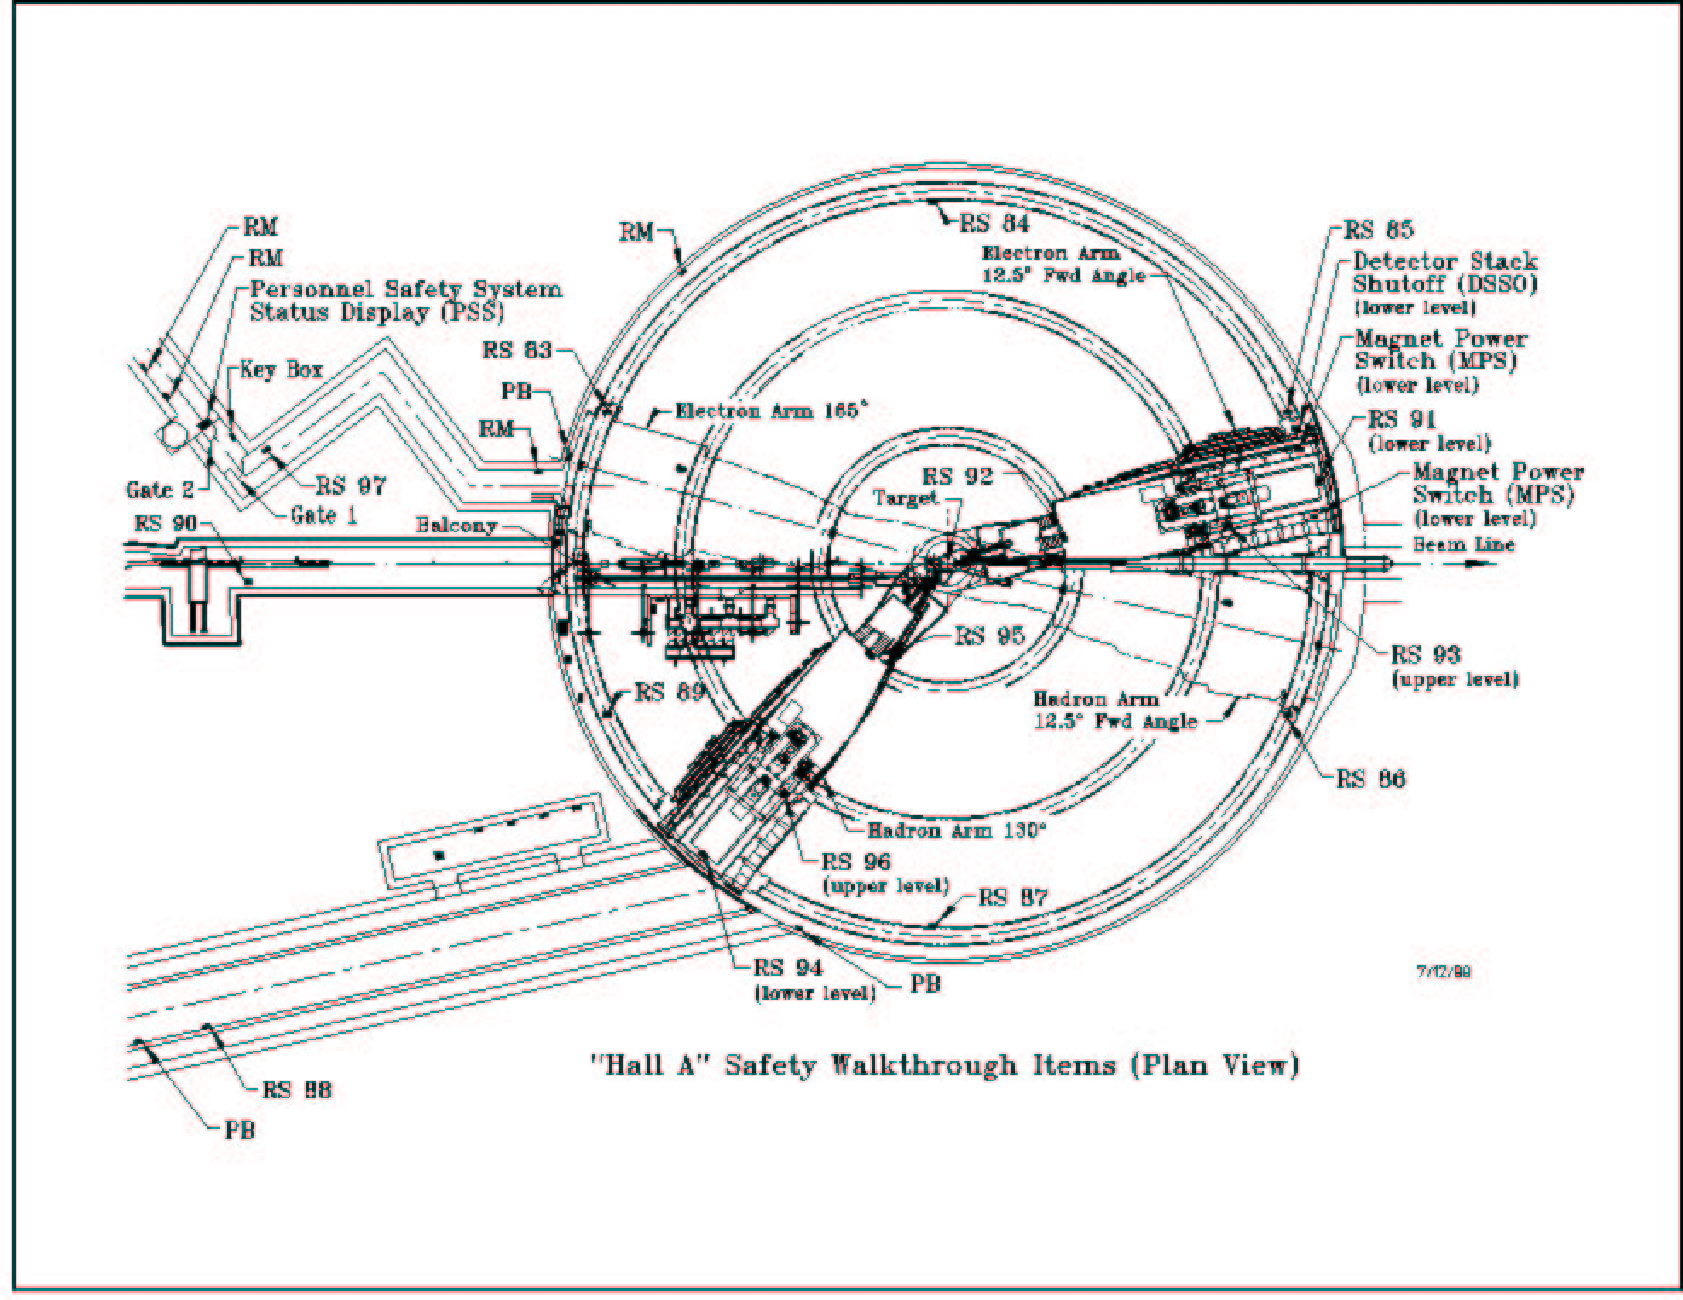
\includegraphics[angle=0,width=15cm]{asafe}
{\linespread{1.}
\caption[Introduction: Location of Hall Safety Items ]{Schematic
of the Hall A showing the location of various safety system
components. The abbreviations are: Radiation Monitor, RM, Run
Safe Box, RS, Fire Alarm Pull Box, PB. }
\label{fig:asafe}}
\end{center}
\end{figure}

\begin{figure}
\begin{center}
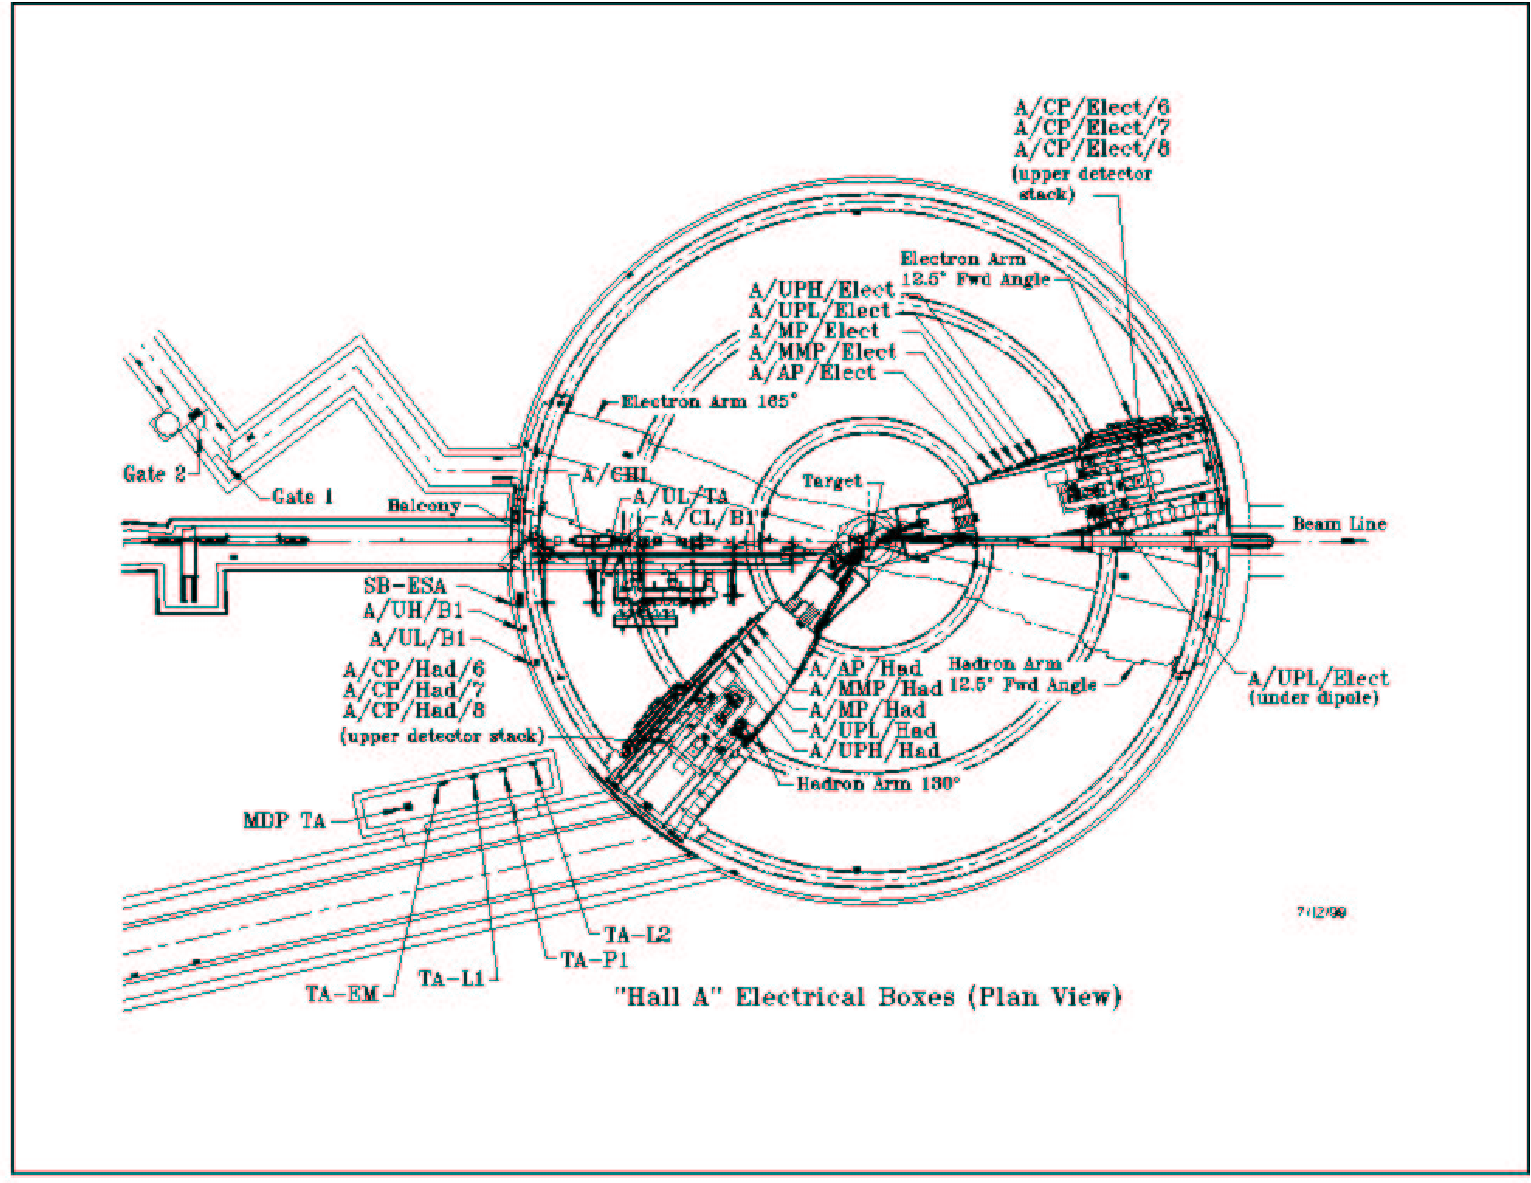
\includegraphics[angle=0,width=15cm]{aelec}
{\linespread{1.}
\caption[Introduction: Location of Circuit Breakers]{Schematic of
the Hall A showing the location of the circuit breaker panels.}
\label{fig:aelec}}
\end{center}
\end{figure}
% ===========  CVS info
% $Header: /group/halla/analysis/cvs/tex/osp/src/introduction/a-intro.tex,v 1.2 2003/11/18 19:52:19 lerose Exp $
% $Id: a-intro.tex,v 1.2 2003/11/18 19:52:19 lerose Exp $
% $Author: lerose $
% $Date: 2003/11/18 19:52:19 $
% $Name:  $
% $Locker:  $
% $Log: a-intro.tex,v $
% Revision 1.2  2003/11/18 19:52:19  lerose
% small change
%
% Revision 1.1  2003/06/06 15:26:26  gen
% Revision printout changed
%
% Revision 1.3  2003/06/06 14:36:44  gen
% Revision printout changed
%
% Revision 1.2  2003/06/05 23:30:01  gen
% Revision ID is printed in TeX
%
% Revision 1.1.1.1  2003/06/05 17:28:28  gen
% Imported from /home/gen/tex/OSP
%
%  Revision parameters to appear on the output
